\documentclass[final]{beamer}
\usetheme{RJH}
\usepackage[orientation=portrait,size=a0,scale=1.4,debug]{beamerposter}
\usepackage[absolute,overlay]{textpos}
\setlength{\TPHorizModule}{1cm}
\setlength{\TPVertModule}{1cm}

\title{Voice Control for a Gripper Using Mel Frequency Cepstral Coefficents and Gaussian Mixture Models}
\author{Velasco-Hernandez, Gustavo $^{1}$. D\'{i}az-Toro, Andr\'{e}s Alejandro $^{2}$}
\institute{Perception and Intelligent Systems Research Group\\
	School of Electric and Electronics Engineering\\
	Universidad del Valle}
\footer{Contact:\\ 1 velasco.gustavo@correounivalle.edu.co\\ 2 andres.a.diaz@correounivalle.edu.co}
\date{}

\begin{document}
\begin{frame}{}

\begin{textblock}{5}(3,3)

\includegraphics[width=0.10\paperwidth]{figs/univalle.png}
\end{textblock}
\begin{textblock}{5}(70,5.5)

\includegraphics[width=0.15\paperwidth]{figs/psilogo3.png}
\end{textblock}


\begin{textblock}{39.5}(1,21)
\begin{block}{Abstract}
This work presents an implementation of a speaker-dependent speech recognition system used to control a gripper. The application was made using MATLAB and the gripper was assembled using the Lego Mindstorm NXT robotic kit. Four commands are implemented for controlling the gripper: Open, close, rotate left and rotate right. The development was divided into two stages. In training stage, we use Mel Frequency Cepstral Coefficients (MFCCs) and Gaussian Mixture Models (GMMs) to generate a representation of each defined command. Then, in testing stage, those models are used to identify the speaker’s utterance and send the command to the actuator. Finally, we present test results that show a performance of 95.09\% for our system, and then we compare it with similar works.
\end{block}

\begin{block}{Training Stage}
\begin{figure}[!ht]
\begin{center}
   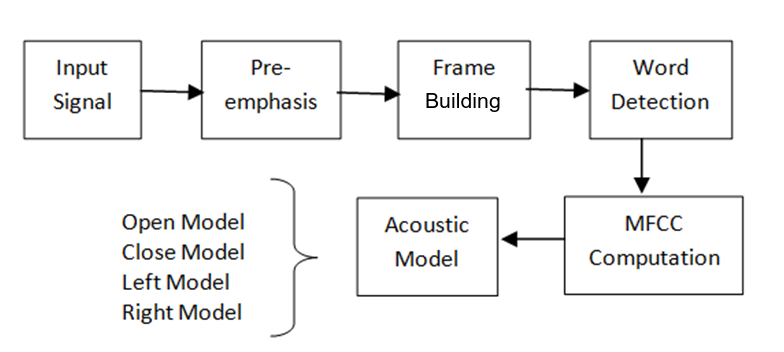
\includegraphics[width=0.8\linewidth]{figs/1bloquesTraining}
\end{center}
   \caption{Blocks for Training Stage.}
\label{trainingBlocks}
\end{figure}
\end{block}

\begin{block}{Testing Stage}
\begin{figure}[!ht]
\begin{center}
   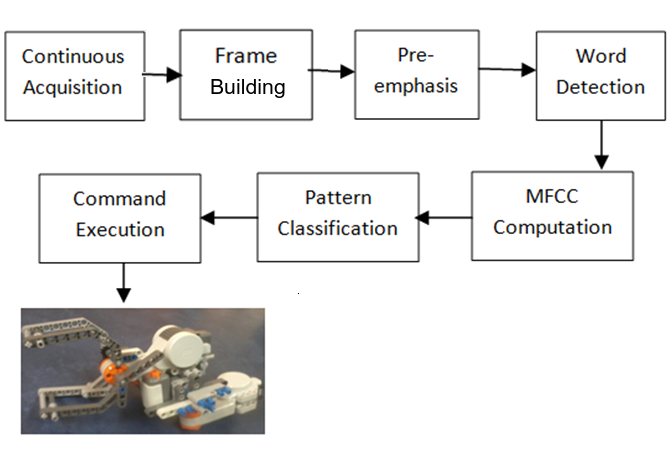
\includegraphics[width=0.8\linewidth]{figs/11bloquesTesting}
\end{center}
   \caption{Blocks for Testing Stage.}
\label{trainingBlocks}
\end{figure}
\end{block}


\end{textblock}

\begin{textblock}{39.5}(43.05,21)
\begin{block}{My latest paper about frogs}
Published in the \emph{Journal of Irreproducible Results}.
\end{block}

\begin{block}{Conclusions}
In this paper we presented an speaker-dependent speech recognition system based on Mel Frequency Cepstral Coefficients (MFCCs) for extracting features and Gaussian Mixture Models (GMMs) for creating the model of each command. We test the systems with two different speakers and the worst case was $91.17\%$ (average of global performance for speaker $1$) of accuracy for a speaker. For a particular command, the worst case was $82.35\%$ and the average of the global performance of the system was $95.09\%$ (see Results section).

As future work, we propose the evaluation of the system with more than four commands and the creation of models with utterances from different speakers in order to test the capability of the system to be speaker-independent.
\end{block}
\end{textblock}

\end{frame}
\end{document}
